\documentclass[aspectratio=169]{beamer}
\usepackage[spanish]{babel}
\usepackage{tikz}
\usepackage{graphicx}
\usepackage{algorithm}
\usepackage{algorithmic}

\usepackage{caption}

\usecolortheme{whale}
\usetikzlibrary{er,positioning}  
\usetikzlibrary{decorations.pathreplacing}
\usetikzlibrary{arrows, decorations.markings}
\usetikzlibrary{shapes.geometric}

\setbeamertemplate{navigation symbols}{}

% \setbeameroption{show notes on second screen=right}

\definecolor{violet}{rgb}{0.53, 0.0, 0.69}

\definecolor{blue1}{RGB}{126,126,206}
\definecolor{blue2}{RGB}{87,87,192}
\definecolor{blue3}{RGB}{51,51,178}
\definecolor{blue4}{RGB}{27,26,107}

\tikzstyle{every link} = []
\tikzstyle{link} = [>=triangle 60, draw, every link]

\definecolor{attr}{RGB}{10,153,2}

\title{Bases de Datos}
\subtitle{Dependencias Funcionales y Anomal\'ias}
\author[Garc\'ia L., Cardentey V. M., Ledesma A.]{
    Lic. Andy Ledesma Garc\'ia\\
    Lic. V\'ictor M. Cardentey Fundora\\ 
    Dra. C. Lucina Garc\'ia Hern\'andez
}
\institute[MATCOM-UH]{
    Departamento de Computaci\'on\\
    Facultad de Matem\'atica y Computaci\'on\\
    Universidad de La Habana\\[3mm]
    Licenciatura en Ciencia de Datos
}
\date[]{13 de febrero de 2024}


\begin{document}
    \maketitle
    


\begin{frame}{Objetivos}
    \begin{block}{Lo que usted aprender\'a}
    \begin{enumerate}[<+->]
        \item Reconocer las restricciones de integridad en un escenario y representarlas adecuadamente en una base de datos relacional.  

        \item Detectar anomal\'ias en una base de datos relacional. 
        % \item Identificar las formas normales en una base de datos relacional. 
        % \item Aplicar algoritmos que permiten determinar las llaves candidatas y la equivalencia entre relaciones.
        % \item Poder obtener un dise\~no de base de datos relacional en tercera forma normal.
    \end{enumerate}
    \end{block}
\end{frame}


{
\setbeamertemplate{background} 
{
    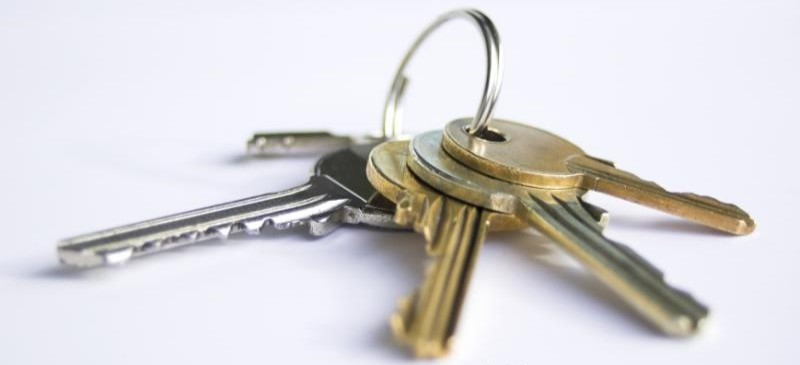
\includegraphics[width=\paperwidth,height=\paperheight]{img/the-keys-to.jpg}
}
\begin{frame}
\end{frame}
}



\begin{frame}{¿Qu\'e es una llave candidata?}
    \begin{block}<2>{Llave candidata}
        Un conjunto de uno o m\'as atributos $K = \{A_1,A_2,...,A_n\}$ es una llave candidata
        de la relaci\'on $R$ si cumple las siguiente propiedades:
        \begin{enumerate}
            \item \textbf{Unicidad}: En cualquier momento dado, no existen dos tuplas
            distintas de $R$ con los mismos valores para $A_1,A_2,...,A_n$.
            \item \textbf{Minimalidad}: Ning\'un subconjunto propio de $K$ tiene la
            propiedad de unicidad.
        \end{enumerate}
    \end{block}
\end{frame}

\begin{frame}
    \centering
    \LARGE \textcolor{blue3}{¿Cómo encontrar las llaves candidatas de una relaci\'on?}
\end{frame}


\begin{frame}{La idea es muy f\'acil}

    Sea $U = \{A_1,...,A_n\}$ el conjunto universo de los atributos de una relaci\'on $R$,

    por cada subconjunto de atributos $X \subseteq U$ comprobar la unicidad y minimalidad.
\end{frame}

\begin{frame}{Minimalidad}
    Un conjunto $C$ es minimal con respecto a una propiedad $P$ si y s\'olo si:\begin{enumerate}
        \item $P(C)$
        \item $\not \exists C' \subset C : P(C')$
    \end{enumerate}
    \vspace{5mm}

    \centering
    \onslide<2>{\Large \textcolor{red}{ Para comprobar la minimalidad debemos comprobar la unicidad}}
\end{frame}


\begin{frame}{Unicidad}
    \centering
    \LARGE ¿Qué es la unicidad?
\end{frame}

\begin{frame}{Unicidad}
    Sea $K = \{A_1,A_2,...,A_n\}$ un conjunto de atributos de
    una relaci\'on $R$, en cualquier momento dado, no existen dos tuplas
    distintas de $R$ con los mismos valores para $A_1,A_2,...,A_n$.
    \vspace{4mm}

    \onslide<2>{
    \centering
    \begin{tikzpicture}
        \node at (0,2) {LLAVE};
        \draw (0,0) node[ellipse, minimum height=3cm,minimum width=2.4cm,draw] {};
        \node at (5,2) {CUERPO};
        \draw (5,0) node[ellipse, minimum height=3cm,minimum width=2.4cm,draw] {};

        \node[circle,fill=black, inner sep=2pt] (k1) at (0,1) {};
        \node[circle,fill=black, inner sep=2pt] (k2) at (0.5,0.5) {};
        \node[circle,fill=black, inner sep=2pt] (k3) at (0,0) {};
        \node[circle,fill=black, inner sep=2pt] (k4) at (0.5,-0.5) {};
        \node[circle,fill=black, inner sep=2pt] (k5) at (0,-1) {};

        \node[circle,fill=black, inner sep=2pt] (p1) at (5,1) {};
        \node[circle,fill=black, inner sep=2pt] (p2) at (4.5,0.5) {};
        \node[circle,fill=black, inner sep=2pt] (p3) at (5,0) {};
        \node[circle,fill=black, inner sep=2pt] (p4) at (4.5,-0.5) {};
        \node[circle,fill=black, inner sep=2pt] (p5) at (5,-1) {};

        \draw (k1) -- (p1);
        \draw (k2) -- (p2);
        \draw (k3) -- (p3);
        \draw (k4) -- (p4);
        \draw (k5) -- (p5);

        
      
    \end{tikzpicture}
    }
\end{frame}


\begin{frame}{Unicidad}
    Sea $K = \{A_1,A_2,...,A_n\}$ un conjunto de atributos de
    una relaci\'on $R$, en cualquier momento dado, no existen dos tuplas
    distintas de $R$ con los mismos valores para $A_1,A_2,...,A_n$.
    \vspace{4mm}

    \centering
    \begin{tikzpicture}
        \node at (0,2) {LLAVE};
        \draw (0,0) node[ellipse, minimum height=3cm,minimum width=2.4cm,draw] {};
        \node at (5,2) {CUERPO};
        \draw (5,0) node[ellipse, minimum height=3cm,minimum width=2.4cm,draw] {};

        \node[circle,fill=black, inner sep=2pt] (k1) at (0,1) {};
        \node[circle,fill=black, inner sep=2pt] (k2) at (0.5,0.5) {};
        \node[circle,fill=black, inner sep=2pt] (k3) at (0,0) {};
        \node[circle,fill=black, inner sep=2pt] (k4) at (0.5,-0.5) {};
        \node[circle,fill=black, inner sep=2pt] (k5) at (0,-1) {};

        \node[circle,fill=black, inner sep=2pt] (p1) at (5,1) {};
        \node[circle,fill=black, inner sep=2pt] (p2) at (4.5,0.5) {};
        \node[circle,fill=black, inner sep=2pt] (p3) at (5,0) {};
        \node[circle,fill=black, inner sep=2pt] (p4) at (4.5,-0.5) {};


        \draw (k1) -- (p1);
        \draw (k2) -- (p2);
        \draw (k3) -- (p3);
        \draw (k4) -- (p4);
        \draw[color=red] (k5) -- (p4);

        
      
    \end{tikzpicture}
    

    \vspace{3mm}

    \centering
    \Large \textcolor{red}{No necesariamente es una funci\'on inyectiva}

    \note{@NOTE destacar q puede haber varias llaves candidatas a primaria}
\end{frame}






\begin{frame}{¿Esta definici\'on ayuda a obtener un algoritmo?}
    Determinar la existencia de una funci\'on entre dos conjuntos de elementos desconocidos
    
    \vspace{5mm}

    \onslide<2>{
        \centering
        \Large \textcolor{red}{¿C\'omo podemos hacer esto?}
    }
\end{frame}


\begin{frame}{Ya sabemos que existen algunas}
    \begin{itemize}
        \item Los proveedores de correo (Google, Yahoo, Outlook, etc.) asocian al
        correo algunos datos personales como el nombre y apellido.
        \item Existe un convenio internacional en el que los pa\'ises acuerdan c\'odigos para
        identificar la ubicaci\'on geogr\'afica (c\'odigo postal).
    \end{itemize}
    \vspace{5mm}

    \onslide<2>{

        Si se desea desarrollar un sistema que requiera tanto los datos personales como la
        ubicaci\'on geogr\'afica del usuario, cu\'al ser\'ia la llave primaria de la relaci\'on Usuario.
    }

\end{frame}


\begin{frame}{Buscando una llave candidata}
    \centering
    \textbf{Usuario}(Email, Nombre, Apellido, C. Postal, Provincia, Pa\'is)
    \vspace{5mm}
    
    \begin{itemize}
        \item<2->  Si conocemos el email de un usuario tambi\'en conocemos su nombre y apellido.
        $$
        \textnormal{Email} \to \textnormal{Nombre, Apellido}
        $$
        \item<3->  Si conocemos el c\'odigo postal de un usuario tambi\'en conocemos su provincia y pa\'is.
        $$
        \textnormal{C. Postal} \to \textnormal{Provincia, Pa\'is}
        $$
    \end{itemize}
    \vspace{5mm}
    
    \onslide<4>{

        \Large \textcolor{red}{¿Cu\'al ser\'ia una llave candidata de esta relaci\'on?}
    }
\end{frame}

\begin{frame}{¿Y si componemos las funciones que ya conocemos?}

    $$
        \textnormal{Email, C. Postal} \to \textnormal{Nombre, Apellido, Provincia, Pa\'is}
    $$
    \vspace{2mm}

    \onslide<2->{

        \begin{itemize}
            \item Supongamos un usuario con email luis.fonseca@gmail.com
            $$
                \textnormal{luis.fonseca@gmail.com} \to \textnormal{Luis, Fonseca}
            $$
            \item Supongamos que tiene el c\'odigo zip 10400
            $$
                \textnormal{10400} \to \textnormal{La Habana, Cuba}
            $$
        \end{itemize}
    }

    \onslide<3>{

        $$\textnormal{luis.fonseca@gmail.com, 10400} \to \textnormal{Luis, Fonseca, La Habana, Cuba}$$
    }

\end{frame}


% \begin{frame}{¿Y si componemos las funciones que ya conocemos?}

%     $$
%         \textnormal{Email, C. Postal} \to \textnormal{Nombre, Apellido, Provincia, Pa\'is}
%     $$
%     \vspace{2mm}

%     \begin{itemize}
%         \item Supongamos un usuario con email luis.fonseca@gmail.com
%         $$
%             \textnormal{luis.fonseca@gmail.com} \to \textnormal{Luis, Fonseca}
%         $$
%         \item Supongamos que tiene el c\'odigo zip 10400
%         $$
%             \textnormal{10400} \to \textnormal{La Habana, Cuba}
%         $$
%     \end{itemize}

    
%     $$\textnormal{luis.fonseca@gmail.com, 10400} \to \textnormal{Luis, Fonseca, La Habana, Cuba}$$

% \end{frame}


\begin{frame}{Dependencia Funcional}
  

    Dada una relaci\'on $R$ y los atributos $X$, $Y$ de $R$, se dice que $Y$ depende funcionalmente de $X$ si
    y s\'olo si el valor de $X$ en cada tupla de $R$ determina el valor
    de $Y$ en dicha tupla. Se representa como $R.X \to R.Y$ o simplemente

    \begin{Huge}
        
        $$
            X \to Y
        $$
    \end{Huge}

    \begin{block}{Notaci\'on}
        \begin{itemize}
            \item Atributo simple: $A,B,C,D,E$
            \item Atributo compuesto (conjunto de atributos simples): $W,X,Y,Z$
        \end{itemize}
    \end{block}
\end{frame}


\begin{frame}{Cumplimiento de una Dependencia Funcional}
    \begin{columns} 
        \column{0.5\textwidth}
        \begin{block}<2->{Funci\'on $f$}
            $$
            x_1 = x_2 \implies f(x_1) = f(x_2)
            $$
        \end{block}
        \begin{block}<3->{Dependencia Funcional $X \to Y$}
            $$
            t_1[X] = t_2[X] \implies t_1[Y] = t_2[Y] 
            $$
        \end{block}

        \column{0.5\textwidth}
        \centering
        \only<4->{
        \begin{tabular}{|c|c|c|}
            \hline
            \underline{\#E} & Grupo & Provincia \\[1mm]
            \hline
            1 & 211 & Pinar del R\'io \\
            2 & \textcolor<8->{red}{212} & \textcolor<8->{red}{La Habana} \\
            3 & \textcolor<8->{red}{213} & \textcolor<8->{red}{La Habana} \\
            15 & 211 & Pinar del R\'io \\
            \hline
        \end{tabular}
        }
        \vspace{5mm}

        \begin{itemize}
            \item<5-> \#E $\to$ Grupo, Provincia
            \item<6-> Grupo $\to$ Provincia
        \end{itemize}
        \vspace{5mm}

        \only<7->{\textcolor{red}{?`Provincia $\to$ Grupo?}}
    \end{columns}
    % Sean 
    % $U = A_1,...,A_n$ el universo de atributos de la
    % relaci\'on $R$, $X \subseteq U$ y $Y \subseteq U$. La dependencia
    % funcional $X \to Y$ se cumple en $R$ si para toda instancia $r(R)$ para todos
    % los pares de tuplas $t_1$ y $t_2$ en $r$ se cumple que:

    % $$
    %     t_1[X] = t_2[X] \implies t_1[Y] = t_2[Y] 
    % $$

    \note<1>{@NOTE ?`qu\'e es lo esencial de las funciones?}
\end{frame}

\begin{frame}{¿C\'omo representar una relaci\'on?}
    \begin{block}{Esquema relacional}
        Un \textbf{esquema relacional} expresado por $R(U,F)$
        constituye una manera abreviada de representar
        la descripci\'on de una relaci\'on mediante: 
        \begin{itemize}
            \item Su nombre $R$.
            \item El conjunto de atributos que la componen $U$, denominado universo de la relaci\'on.
            \item El conjunto de dependencias funcionales $F$ que se cumple en $R$.
        \end{itemize}
    \end{block}
    
    \note{@NOTE funciones entre los datos}
\end{frame}

\begin{frame}{Utilidad de las dependencias funcionales}
    \begin{itemize}
        \item<1-> Especificar las restricciones en el conjunto de instancias
        legales de una relaci\'on $R$ 
        (instancias $r$ de $R$ que satisfacen un conjunto de dependencias funcionales $F$):\\ 
        \centering \textcolor{red}{F se cumple en R}\vspace{2mm}
        \item<2-> Probar si una instancia $r$ de una relaci\'on $R$ es legal bajo un conjunto de
        dependencias funcionales $F$:\\
        \centering \textcolor{red}{r satisface a F} \vspace{2mm}
        \item<3-> ¿Y los algoritmos?
    \end{itemize}

    \note<2>{@NOTE hacer \'enfasis en la 2da q es la q + le interesa a ellos, pa saber si lo q existe esta' bien representado}
\end{frame}

{
\setbeamertemplate{background} 
{
    
\includegraphics[width=\paperwidth,height=\paperheight]{img/automate.jpg}
}
\begin{frame}
\end{frame}
}





\begin{frame}{Ejemplo de aplicaci\'on del algoritmo para comprobar la unicidad}
    Sea $R(U,F)$ con:
    \begin{itemize}
        \item $U = \{A,B,C,D,E,G\}$
        \item $F = \{AB \to C, {\color<3>{red}C} \to A, BC \to D, {\color<5>{red}ACD} \to B, {\color<7>{red}D} \to EG, BE \to C \}$
    \end{itemize}
    comprobar si $CD$ cumple la unicidad.
    \vspace{4mm}
    
    \onslide<2->{

        Inicializamos $X_0 = {\color<3>{red}C}D$
        \begin{enumerate}
            \item<4-> $X_1 = {\color<5>{red}ACD}$
            \item<6-> $X_2 = ABC{\color<7>{red}D}$
            \item<8-> $X_3 = ABCDEG$
        \end{enumerate}
        \onslide<9>{$X_3 = U$, se cumple la unicidad} 
    }
\end{frame}


\begin{frame}{Formalizando}

    \begin{block}{Implicaci\'on l\'ogica}
        Sea un esquema relacional $R(U,F)$ y $X \to Y$ una dependencia funcional. Se dice
        que $F$ implica l\'ogicamente a $X \to Y$ o que $X \to Y$ se
        deduce l\'ogicamente de $F$ si cada instancia $r$ de $R$ que
        satisfaga las dependencias funcionales en $F$ tambi\'en satisface $X \to Y$.

        $$
            F \models X \to Y
        $$
    \end{block}

\end{frame}


\begin{frame}{Clausura de un conjunto de atributos}
    Sea un esquema relacional $R(U,F)$, un conjunto de atributos
    $X$ tal que $X \subseteq U$.
    La clausura del conjunto de atributos $X$ con respecto a un conjunto
    de dependencias funcionales $F$ -- denotada por $X^+_F$ o abreviadamente $X^+$--
    es el conjunto de atributos simples que se determina funcionalmente por $X$ a partir
    de las dependencias funcionales de $F$.

    $$
        X^+_F = \{ A_i \in U \;|\; F \models X \to A_i\}
    $$
\end{frame}


\begin{frame}{Mejorando la definici\'on de llave candidata}
    Sea $K$ un conjunto de atributos $\{A_1, A_2, ..., A_n\}$ de una esquema
    relacional $R(U,F)$ es llave candidata candidata del esquema
    si cumple las siguientes propiedades:
    \begin{enumerate}
        \item \textbf{Unicidad}: $K^+_F = U$
        \item \textbf{Minimalidad}: Ning\'un subconjunto propio de $K$ tiene la propiedad de unicidad.
    \end{enumerate}
    
    
\end{frame}

\begin{frame}{Mejorando el algoritmo para comprobar la unicidad}

    El conjunto de atributos $X$ cumple la unicidad en $R(U,F)$ si y s\'olo si $X^+_F = U$ 
\end{frame}


\begin{frame}{¿Qu\'e herramientas podemos aplicar para inferir l\'ogicamente?}
    \onslide<2>{
        
        \begin{block}{Axiomas de Inferencia (Armstrong, 1974)}
            Sea un esquema relacional $R(U,F)$:
            \begin{enumerate}
                \item \textbf{Reflexividad}: Si $Y \subseteq X \subseteq U$, entonces $X \to Y$
                se deduce l\'ogicamente de $F$.
                \item \textbf{Aumentatividad}: Si se cumple que $X \to Y$ y $Z \subseteq U$, entonces
                $XZ \to YZ$.
                \item \textbf{Transitividad}: Si se cumple que $X \to Y$ y $Y \to Z$, entonces $X \to Z$. 
            \end{enumerate}
    
        \end{block}
        \vspace{5mm}
    
        \begin{footnotesize}
            Armstrong, W. W. [1974]. \textit{``Dependency structures of data base relationships,''}\\
            Proc. 1974 IFIP Congress, pp. 580-583, North Holland, Amsterdam.
        \end{footnotesize}
    }
\end{frame}

\begin{frame}{Lemas derivados}
    Sea un esquema relacional $R(U,F)$:
    \begin{enumerate}
        \item \textbf{Composici\'on}: $\{X \to Y, W \to Z \;|\; W \subseteq X\} \models X \to YZ$ 
        \item \textbf{Descomposici\'on}: $\{X \to Y, Z \subseteq Y\} \models X \to Z$
        \item \textbf{Pseudotransitividad}: $\{ X \to Y, WY \to Z \}  \models XW \to Z$
    \end{enumerate}
\end{frame}


\begin{frame}{Clausura de un conjunto de dependencias funcionales}
    Sea un esquema relacional $R(U,F)$. La clausura del conjunto
    de dependencias $F$ \\ -- denotada por $F^+$ -- es el conjunto de las
    dependencias funcionales implicadas l\'ogicamente por $F$. Formalmente,
    se define como:
    
    $$
        F^+=\{ X \to Y \;|\; F \models X \to Y \}
    $$

    \note{@NOTE llamar la atenci\'on sobre la dif entre $X->Y \in F$ y $F \models X->Y$ }
\end{frame}


\begin{frame}{Trivialidad de una dependencia funcional}    
    Sean $X$ y $Y$ atributos no necesariamente simples, tal que $X \cap Y = \emptyset$.\\[5mm]

    \begin{columns}[t]
        \column{.35\textwidth}
        \centering
        \only<2->{
            $X \to X$

        Trivial}

        \column{.3\textwidth}
        \centering
        \only<3->{$X \to XY$

        No trivial}

        \column{.35\textwidth}
        \centering
        \only<4->{$X \to Y$

        Completamente no trivial}
    \end{columns}

    \note<2>{@NOTE destacar que las triviales son especiales y que siempre est\'an en la clausura}
\end{frame}


\begin{frame}{¿Es viable computar $F^+$?}
    \begin{center}
        \Large
        ¿Cu\'antas dependencias funcionales triviales existen en $F^+$?
    \end{center}

        \only<2->{\large R/ La cantidad de DF's triviales es \textbf{\textcolor{red}{exponencial}} con respecto a la cantidad de atributos en $U$.}

    \onslide<3>{
\begin{center}
\Large
        ¿C\'omo podemos determinar si una dependencia funcional $X \to Y$ pertenece a $F^+$?
\end{center}
    }

    \note<2>{@NOTE no es viable computar F+}
\end{frame}

\begin{frame}{Alternativa: Utilizar la clausura de un conjunto de atributos}

    \onslide<2->{

        La clausura de un conjunto de atributos es $X^+_F = \{ A_i \in U \;|\; F \models X \to A_i\}$
        \vspace{3mm}

    \begin{columns}[t]
        \column<2->{.5\textwidth}

        ¿$X \to Y$ pertenece a $F^+$?
        \begin{enumerate}
            \item Calcular $X^+_F$
            \item Comprobar que $Y \subseteq X^+_F$
        \end{enumerate}

        \column<3->{.5\textwidth}
        \begin{algorithm}[H]
            \caption*{Get $X_F^+$}
            \begin{algorithmic}[1] % The number tells where the line numbering should start
                \STATE $S = \{X\}$
                \STATE $S' = S$\label{algorithm:attribute-clausure:line:S'}
                \FOR{each $W \to Z$ in $F$}
                    \IF{$W \subseteq S$}
                        \STATE $S = S \cup Z$
                    \ENDIF
                \ENDFOR

                \IF{$S \neq S'$}
                    \STATE \textbf{goto} line \ref{algorithm:attribute-clausure:line:S'}
                \ENDIF

                \RETURN $S$
            \end{algorithmic}
        \end{algorithm}
    \end{columns}
    }

    \note{@NOTE es en los 2 sentidos: devuelve true o false si X->Y pertenece a F+}
\end{frame}

\begin{frame}{Equivalencia de conjuntos de dependencias funcionales}

    $$
        F \equiv G \Leftrightarrow F^+ = G^+
    $$

    \begin{itemize}
        \item Se debe considerar cada $X \to Y$ en $F$ y determinar si $X^+_G$ contiene
        a $Y$.
        \item Se debe considerar cada $Z \to W$ en $G$ y determinar si $Z^+_F$ contiene
        a $W$.
    \end{itemize}
\end{frame}


\begin{frame}{Si tenemos el conjunto de DFs del universo de atributos}
    \centering
    \LARGE ¿Podemos garantizar la calidad de la base de datos?
    
\end{frame}
    {
\setbeamertemplate{background} 
{
    
\includegraphics[width=\paperwidth,height=\paperheight]{img/database-issues.jpg}
}
\begin{frame}
\end{frame}
}

\begin{frame}{La situaci\'on}
    Se desea desarrollar una base de datos para registrar las notas
    de los estudiantes de la carrera en cada una de las asignaturas que
    cursan:
    \begin{itemize}
        \item De cada estudiante se conoce su identificador, su nombre, su grupo y su provincia de residencia.
        \item De cada asignatura se conoce su identificador y su nombre.
        \item Por cada asignatura se conoce la nota que obtuvo el estudiante en la evaluaci\'on final.
    \end{itemize}
    Adem\'as, se conoce que los estudiantes son organizados en los grupos de acuerdo a su provincia.
\end{frame}


\begin{frame}{Primero lo primero}

    \resizebox{\linewidth}{!}{
                \begin{tikzpicture}[node distance=6em]
                    \tikzstyle{every entity} = [minimum width=2cm, minimum height=1.2cm]
                    \node[entity] (estudiante) {ESTUDIANTE}
                        [sibling distance=3cm]
                        child {node[attribute] [above right of=estudiante] {\tiny PROVINCIA}}
                        child {node[attribute] [above of=estudiante] {\tiny GRUPO}}
                        child {node[attribute] [above left of=estudiante] {\tiny ENOMBRE}}
                        child {node[attribute] [left of=estudiante] {\underline{\tiny \#E}}};
                  
                    \node[entity] (asignatura) at (8,0) {ASIGNATURA}
                    [sibling distance=3cm]
                    child {node[attribute] [right of=asignatura] {\underline{\tiny \#A}}}
                    child {node[attribute] [above right of=asignatura] {\tiny ANOMBRE}};
                    
                  
                    \node[relationship,aspect=2] (evaluar) at (4,0) {EVALUAR}[node distance=4em]
                    child {node[attribute] [above of=evaluar] {\tiny NOTA}};
                    \draw (evaluar.east) -- (asignatura.west) node[above left] {$0,\ast$};
                    \draw (evaluar.west) -- (estudiante.east) node[above right] {$0,\ast$};
                \end{tikzpicture}
            }
\end{frame}


\begin{frame}{Metodolog\'ia para obtener un esquema relacional correcto}
    \begin{enumerate}
        \item Identificar el universo $U$ de atributos del fen\'omeno.
        \item Identificar el conjunto $F$ de las dependencias funcionales que se establecen entre los atributos.
        \item Definir el esquema relacional $R(U,F)$.
    \end{enumerate}
\end{frame}


\begin{frame}{Ejemplo}
    \begin{enumerate}
        \item $U = \{ \textnormal{\#E, ENombre,  Grupo, Provincia, \#A, ANombre, Nota}\}$
    \end{enumerate}

    \onslide<2>{
    \vspace{10mm}

    \centering    
    \large{¿C\'omo podemos obtener $F$ a partir del dise\~no conceptual?}}
\end{frame}

\begin{frame}{Algoritmo de extracci\'on de dependencias funcionales}
    \begin{enumerate}
        \item<2-> Por cada conjunto de entidades con un conjunto de atributos $X \subseteq U$,
        se a\~nade la dependencia funcional $K \to X$ donde $K$ es la llave del conjunto de entidades.
        \item<3-> Por cada conjunto de interrelaciones se toma su llave $K$ y se a\~nade la
        dependencia funcional $K \to K$. Adem\'as, por cada conjunto de entidades en un extremo
        de cardinalidad m\'axima 1 en la interrelaci\'on, se a\~nade la dependencia funcional $K - K_E \to K_E$ donde
        $K_E$ es la llave del conjunto de entidades.
        \item<4-> Por cada agregaci\'on con un conjunto de atributos $X \subseteq U$ se a\~nade la dependencia
        funcional $K \to X$ donde $K$ es la llave del conjunto de interrelaciones que encierra la agregaci\'on.
        \item<5-> A\~nadir aquellas dependencias funcionales asociadas a otras restricciones del negocio
        especificadas en los requerimientos.
    \end{enumerate}
        
\end{frame}


\begin{frame}{Ejecutando el algoritmo}
    \centering
    \resizebox{!}{2.5cm}{
        \begin{tikzpicture}[node distance=6em]
            \tikzstyle{every entity} = [minimum width=2cm, minimum height=1.2cm]
            \node[entity] (estudiante) {ESTUDIANTE}
                [sibling distance=3cm]
                child {node[attribute] [above right of=estudiante] {\tiny PROVINCIA}}
                child {node[attribute] [above of=estudiante] {\tiny GRUPO}}
                child {node[attribute] [above left of=estudiante] {\tiny ENOMBRE}}
                child {node[attribute] [left of=estudiante] {\underline{\tiny \#E}}};
            
            \node[entity] (asignatura) at (8,0) {ASIGNATURA}
            [sibling distance=3cm]
            child {node[attribute] [right of=asignatura] {\underline{\tiny \#A}}}
            child {node[attribute] [above right of=asignatura] {\tiny ANOMBRE}};
            
            
            \node[relationship,aspect=2] (evaluar) at (4,0) {EVALUAR}[node distance=4em]
            child {node[attribute] [above of=evaluar] {\tiny NOTA}};
            \draw (evaluar.east) -- (asignatura.west) node[above left] {$0,\ast$};
            \draw (evaluar.west) -- (estudiante.east) node[above right] {$0,\ast$};
        \end{tikzpicture}
    }
        \vspace{3mm}


        \begin{enumerate}
            \item<2-> Se tienen los conjuntos de entidades ESTUDIANTE y ASIGNATURA:\begin{itemize}
                \item $\textnormal{\#E} \to \textnormal{ENombre, Grupo, Provincia}$
                \item $\textnormal{\#A} \to \textnormal{ANombre}$
            \end{itemize}
            \item<3-> Se tiene el conjunto de interrelaciones EVALUAR: \begin{itemize}
                \item $\textnormal{\#E,\#A} \to \textnormal{\#E,\#A}$
            \end{itemize}
            \item<4-> Se tiene la agregaci\'on ASIGNATURA-EVALUADA \begin{itemize}
                \item $\textnormal{\#E, \#A} \to \textnormal{Nota}$
            \end{itemize}
            \item<5-> A\~nadimos las restricciones planteadas en la especificaci\'on: \begin{itemize}
                \item $\textnormal{Provincia} \to \textnormal{Grupo}$
            \end{itemize}
        \end{enumerate}
\end{frame}

\begin{frame}{Continuemos con el ejemplo}
    \begin{enumerate}
        \item $U = \{ \textnormal{\#E, ENombre,  Grupo, Provincia, \#A, ANombre, Nota}\}$
        \item $F = \{$ \\
        \hspace{10mm} $\textnormal{\#E} \to \textnormal{ENombre, Grupo, Provincia}$\\
        \hspace{10mm} $\textnormal{\#A} \to \textnormal{ANombre}$\\
        \hspace{10mm} $\textnormal{\#E,\#A} \to \textnormal{\#E,\#A}$\\
        \hspace{10mm} $\textnormal{\#E, \#A} \to \textnormal{Nota}$\\
        \hspace{10mm} $\textnormal{Provincia} \to \textnormal{Grupo}$\\
        $\}$
        \item Definimos el esquema relacional $\textbf{Evaluaciones}(U,F)$ con llave \#E, \#A 
    \end{enumerate}

    \note{@NOTE aki' se pone una trivial expli'citamente (spoiler). Provincia->Grupo es una externa al merx}
\end{frame}

\begin{frame}{¿Es este un buen dise\~no? (Anomal\'ia de inserci\'on)}
    \centering
    \begin{tabular}{ccccccc}
        \underline{\#E} & ENombre & Grupo & Provincia & \underline{\#A} & ANombre & Nota\\
        $e_1$ & Juan & {111} & { La Habana} & $a_1$ & An\'alisis & 3\\
        $e_1$ & Juan & {111} & { La Habana} & $a_2$ & L\'ogica & 2\\
        $e_1$ & Juan & {111} & { La Habana} & $a_3$ & \'Algebra & 4\\
        $e_1$ & Juan & {111} & { La Habana} & $a_4$ & Programaci\'on & 5\\
        $e_3$ & Pedro & {111} & { La Habana} & $a_3$ & \'Algebra & 4\\
        $e_2$ & Mar\'ia & {112} & { Matanzas} & $a_1$ & An\'alisis & 3\\
        $e_2$ & Mar\'ia &  {112} & { Matanzas} & $a_2$ & L\'ogica & 3\\
        $e_4$ & Rita &  {112} & { Mayabeque} & $a_2$ & L\'ogica & 3\\
        $e_4$ & Rita &  {112} & { Mayabeque} & $a_4$ & Programaci\'on & 4\\
        $e_5$ & Carlos &  {113} & { Pinar del R\'io} & $a_3$ & \'Algebra & 3
    \end{tabular}
    \vspace{5mm}

    \centering
    \only<2,3>{
        {¿Se pudiera insertar un alumno que todav\'ia no ha recibido evaluaciones?}\\[2mm]
        \begin{tabular}{ccccccc}
            {\color<3>{red}$e_6$} & Marcos & 111 & La Habana & {\color<3>{red}NULL} & NULL & NULL
            
        \end{tabular}
        }
\end{frame}

\begin{frame}{¿Es este un buen dise\~no? (Anomal\'ia de eliminaci\'on)}
    \centering
    \begin{tabular}{ccccccc}
        \underline{\#E} & ENombre & Grupo & Provincia & \underline{\#A} & ANombre & Nota\\
        $e_1$ & Juan & 111 & La Habana & $a_1$ & An\'alisis & 3\\
        $e_1$ & Juan & 111 & La Habana & $a_2$ & L\'ogica & 2\\
        $e_1$ & Juan & 111 & La Habana  & $a_3$ & \'Algebra & 4\\
        $e_1$ & Juan & 111 & La Habana & $a_4$ & Programaci\'on & 5\\
        $e_3$ & Pedro & 111 & La Habana & $a_3$ & \'Algebra & 4\\
        $e_2$ & Mar\'ia & 112 &  Matanzas & $a_1$ & An\'alisis & 3\\
        $e_2$ & Mar\'ia &  112 & Matanzas & $a_2$ & L\'ogica & 3\\
        $e_4$ & Rita & 112 & Mayabeque & $a_2$ & L\'ogica & 3\\
        $e_4$ & Rita &  112 & Mayabeque & $a_4$ & Programaci\'on & 4\\
        \onslide<-1>{
        $e_5$ & Carlos &  113 & Pinar del R\'io & $a_3$ & \'Algebra & 3
        }
    \end{tabular}
    \vspace{5mm}

    \only<1>{
        ¿Qu\'e ocurre si se eliminan las notas del estudiante $e_5$?
    }
    \only<2>{
        \textcolor{red}{Se pierde la informaci\'on relacionada con la provincia Pinar del R\'io y el grupo C113}
    }

\end{frame}


\begin{frame}{¿Es este un buen dise\~no? (Anomal\'ia de modificaci\'on)}
    \centering
    \begin{tabular}{ccccccc}
        \underline{\#E} & ENombre & Grupo & Provincia & \underline{\#A} & ANombre & Nota\\
        $e_1$ & Juan & 111 & {\color<2>{red} La Habana} & $a_1$ & An\'alisis & 3\\
        $e_1$ & Juan & 111 & {\color<2>{red} La Habana} & $a_2$ & L\'ogica & 2\\
        $e_1$ & Juan & 111 & {\color<2>{red} La Habana} & $a_3$ & \'Algebra & 4\\
        $e_1$ & Juan & 111 & {\color<2>{red} La Habana} & $a_4$ & Programaci\'on & 5\\
        $e_3$ & Pedro & 111& La Habana & $a_3$ & \'Algebra & 4\\
        $e_2$ & Mar\'ia & 112 & Matanzas & $a_1$ & An\'alisis & 3\\
        $e_2$ & Mar\'ia &  112 &  Matanzas & $a_2$ & L\'ogica & 3\\
        $e_4$ & Rita &  112 & Mayabeque & $a_2$ & L\'ogica & 3\\
        $e_4$ & Rita &  112 & Mayabeque & $a_4$ & Programaci\'on & 4\\
        $e_5$ & Carlos &  113 & Pinar del R\'io & $a_3$ & \'Algebra & 3
    \end{tabular}
    \vspace{5mm}

    \only<1>{
        ¿Qu\'e tendr\'iamos que hacer si queremos cambiar la provincia de Juan?
    }
    \only<2>{
        \textcolor{red}{Todas las tuplas deben ser modificadas en una misma transacci\'on}
    }
\end{frame}

\begin{frame}
    \frametitle{?`Es este un buen dise\~no? (Redundacia)}

    \centering
    \begin{tabular}{ccccccc}
        \underline{\#E} & ENombre & Grupo & Provincia & \underline{\#A} & ANombre & Nota\\
        $e_1$ & Juan & {\color{orange}111} & {\color{orange} La Habana} & $a_1$ & An\'alisis & 3\\
        $e_1$ & Juan & {\color{orange}111} & {\color{orange} La Habana} & $a_2$ & L\'ogica & 2\\
        $e_1$ & Juan & {\color{orange}111} & {\color{orange} La Habana} & $a_3$ & \'Algebra & 4\\
        $e_1$ & Juan & {\color{orange}111} & {\color{orange} La Habana} & $a_4$ & Programaci\'on & 5\\
        $e_3$ & Pedro & {\color{orange}111} & {\color{orange} La Habana} & $a_3$ & \'Algebra & 4\\
        $e_2$ & Mar\'ia & {\color{blue}112} & {\color{blue} Matanzas} & $a_1$ & An\'alisis & 3\\
        $e_2$ & Mar\'ia &  {\color{blue}112} & {\color{blue} Matanzas} & $a_2$ & L\'ogica & 3\\
        $e_4$ & Rita &  {\color{blue}112} & {\color{blue} Mayabeque} & $a_2$ & L\'ogica & 3\\
        $e_4$ & Rita &  {\color{blue}112} & {\color{blue} Mayabeque} & $a_4$ & Programaci\'on & 4\\
        $e_5$ & Carlos &  {\color{green}113} & {\color{green} Pinar del R\'io} & $a_3$ & \'Algebra & 3
    \end{tabular}
    \vspace{5mm}

    \centering
    {\textcolor{red}{¿Es necesaria esta redundancia?}}
\end{frame}








\begin{frame}{Entonces...}
    \centering
    \Large ¿C\'omo solucionar estas anomal\'ias?
\end{frame}

\begin{frame}{F\'acil...}
    \begin{columns}[T]
        \begin{column}{0.68\linewidth}
            \begin{columns}[T]
                \begin{column}{0.6\textwidth}
                    \begin{center}
                        \textbf{Estudiante}\\[2mm]
        
                        \begin{tabular}{ccc}
                            \underline{\#E} & ENombre & Provincia\\[1mm]
                            \hline
                            $e_1$ & Juan & La Habana\\
                            $e_2$ & Mar\'ia & Matanzas\\
                            $e_3$ & Pedro & La Habana\\
                            $e_4$ & Rita & Mayabeque\\
                            $e_5$ & Carlos & Pinar del R\'io
                        \end{tabular}
                    \end{center}
                \end{column}

                \begin{column}{0.4\textwidth}
                    \begin{center}
                        \textbf{Provincia-Grupo}\\[2mm]
        
                        \begin{tabular}{cc}
                            \underline{Provincia} & Grupo\\[1mm]
                            \hline
                            La Habana & 111\\
                            Matanzas & 112 \\
                            Mayabeque & 112 \\
                            Pinar del R\'io & 113
                            
                        \end{tabular}
                    \end{center}
                \end{column}
                
            \end{columns}

            \begin{center}
                \textbf{Asignatura}\\[2mm]

                \begin{tabular}{cc}
                    \underline{\#A} & ANombre\\[1mm]
                    \hline
                    $a_1$ & An\'alisis\\
                    $a_2$ & L\'ogica \\
                    $a_3$ & \'Algebra\\
                    $a_4$ & Programaci\'on
                    
                \end{tabular}
            \end{center}
            
        \end{column}

        \begin{column}{0.3\linewidth}
            \vspace{6mm}
            \begin{center}
                \textbf{Evaluar}\\[2mm]

                \begin{tabular}{ccc}
                    \underline{\#E} & \underline{\#A} & Nota\\[1mm]
                    \hline
                    $e_1$ & $a_1$ & 3\\
                    $e_1$ & $a_2$ & 2\\
                    $e_1$ & $a_3$ & 4\\
                    $e_1$ & $a_4$ & 5\\
                    $e_3$ & $a_3$ & 4\\
                    $e_2$ & $a_1$ & 3\\
                    $e_2$ & $a_2$ & 3\\
                    $e_4$ & $a_2$ & 3\\
                    $e_4$ & $a_4$ & 4\\
                    $e_5$ & $a_3$ & 3\\
                \end{tabular}
            \end{center}
        \end{column}
    \end{columns}
\end{frame}

    \begin{frame}{Formalizando el dise\~no}
        \centering
        \Large{ ¿C\'omo obtener esta soluci\'on?}
        
        \vfill
        
        \hfill
        \begin{minipage}{0.3\textwidth}
            \only<2>{\it continuar\'a...}
        \end{minipage}
    \end{frame}

    \begin{frame}{Entonces...}

    \begin{columns}[T]
        \begin{column}{0.4\linewidth}
            \vspace{3.3cm}

            \Huge ... alguna duda?
        \end{column}
        \begin{column}{0.58\linewidth}
            
            
\includegraphics[height=0.8\textheight, width=\linewidth]{img/doubts.jpg}
        \end{column}
        
    \end{columns}
    
\end{frame}

    \maketitle
    \begin{frame}
    \frametitle{Anexos}

    \centering
    \Huge \textcolor{blue3}{Anexos}

\end{frame}

\begin{frame}{Anexos}
    \framesubtitle{Algoritmo para determinar si un conjunto de atributos cumple la unicidad}

    \textbf{Entrada}: $U = \{A_1,A_2,...,A_n\}$, $F$ conjunto de dependencias funcionales y $X$, $X \subseteq U$\\
    \textbf{Salida}: 1 si el conjunto $X$ cumple la unicidad en $R(U,F)$ o 0 en otro caso.\\
    \textbf{M\'etodo}:
    \begin{enumerate}
        \item Sea $X$ el conjunto de atributos que se desea comprobar. Primero inicializamos
        $X_0 = X$.
        \item En cada iteraci\'on $i$ se busca una dependencia funcional $Y \to A$ tal que
        $Y \subseteq X_{i-1}$, pero $A \notin X_{i-1}$. Entonces
        se asigna $X_i = X_{i-1} \cup \{A\}$.
        \item Repetir el paso 2 tantas veces como sea necesario hasta que no puedan a\~nadirse
        m\'as atributos. Dado que el conjunto resultante solo puede crecer y la cantidad de atributos
        en el universo es finito, eventualmente el algoritmo termina.
        \item Sea $k$ la iteraci\'on final del algoritmo, se comprueba que $X_k = U$.  
        
    \end{enumerate}
\end{frame}
\end{document}
